 \chapter{Marco Teórico}
 \markboth{CAPÍTULO 2. Marco Teórico}{\small CAPÍTULO 2. Marco Teórico}
 \label{MarcoTeorico}

\section{Fundamentos de las bioseñales electromiográficas}

\noindent Las bioseñales son manifestaciones eléctricas derivadas de la actividad fisiológica de los tejidos excitables, tales como músculos, nervios o glándulas. Su registro y análisis permiten inferir el comportamiento dinámico de sistemas biológicos complejos y establecer relaciones cuantitativas entre los procesos bioeléctricos y las respuestas funcionales del organismo. Dentro de este conjunto, las señales electromiográficas (EMG) constituyen un medio experimental esencial para el estudio de la actividad neuromuscular, al reflejar la suma de los potenciales eléctricos generados durante la contracción de fibras musculares bajo control voluntario o reflejo.

En el contexto del sistema urinario inferior, la electromiografía del esfínter externo de la uretra (EEU) se ha consolidado como una herramienta de gran relevancia para comprender los mecanismos fisiológicos que regulan la continencia urinaria y el control miccional. El EEU es un músculo estriado somático que recibe inervación principalmente de las raíces nerviosas lumbosacras (L6–S1). Cuando dichas raíces son lesionadas o avulsionadas, se interrumpe la transmisión motora hacia el esfínter, lo que genera una reducción significativa en la actividad electromiográfica y, en consecuencia, una alteración funcional de la micción (véase [Corona-Quintanilla et al., año]).

El modelo de avulsión lumbosacra en conejas ha permitido reproducir experimentalmente este fenómeno y estudiar la reorganización de los circuitos neurales que intervienen en la función urinaria. Mediante el registro simultáneo de la presión uretral (PU) y la actividad electromiográfica (EMG) durante la aplicación de trenes de estímulos eléctricos controlados, se obtiene una representación precisa de la respuesta neuromuscular del sistema. Dichos registros, segmentados en ventanas de tiempo —Basal, A-inicial, A-mayor y A-final—, contienen información valiosa sobre la evolución temporal de la activación muscular y su modulación fisiológica.

Sin embargo, la naturaleza oscilatoria, ruidosa y no estacionaria de las señales electromiográficas exige la aplicación de métodos matemáticos avanzados para su análisis. Es en este punto donde el procesamiento digital de señales (DSP) y la matemática aplicada convergen como pilares fundamentales del estudio cuantitativo de la fisiología.

\subsection{Procesamiento digital de señales biomédicas}

El procesamiento digital de señales consiste en el conjunto de técnicas matemáticas y computacionales empleadas para adquirir, filtrar, transformar y analizar señales discretizadas en el tiempo. Su objetivo es extraer información relevante y reducir el impacto del ruido o de las variaciones indeseadas presentes en los datos experimentales. En el ámbito biomédico, estas técnicas son esenciales para convertir registros fisiológicos en descripciones cuantitativas útiles para la investigación o la práctica clínica.

Una bioseñal, denotada por $x(t)$, puede representarse en su forma discretizada $x[n]$, donde $n$ indica la secuencia temporal de muestras obtenidas a una frecuencia de muestreo $f_s$. El tratamiento matemático de estas secuencias implica operaciones como la filtración, la detección de picos, la segmentación temporal y, de manera crucial, la transformación de dominio, que permite analizar la señal desde distintas perspectivas.

Entre las herramientas más utilizadas se encuentra la Transformada de Fourier (TF), que expresa una señal en términos de sus componentes sinusoidales de frecuencia. Esta transformación revela la estructura espectral del fenómeno fisiológico, permitiendo estudiar la distribución de energía o amplitud en función de la frecuencia. La Transformada Rápida de Fourier (FFT, Fast Fourier Transform) es una versión computacionalmente eficiente de la TF, capaz de procesar grandes volúmenes de datos con una complejidad algorítmica de orden $O(N \log N)$, donde $N$ es el número de muestras de la señal.

\subsection{Fundamento matemático de la Transformada Rápida de Fourier (FFT}

La Transformada Discreta de Fourier (DFT) de una señal $x[n]$ de longitud $N$ se define como:

\begin{equation}
	X[k] = \sum_{n=0}^{N-1} x[n] e^{\frac{-j2 \pi k n}{N}}, \text{ } \text{ } k = 0,1,...,N-1
\end{equation}

donde $X[k]$ representa los coeficientes complejos que describen la amplitud y fase de las componentes frecuenciales. La FFT optimiza el cálculo de la DFT al reducir el número de operaciones necesarias, lo que la convierte en un método estándar para el análisis espectral en tiempo real.

En el análisis de bioseñales electromiográficas, la FFT permite determinar las frecuencias dominantes asociadas a la actividad muscular, las cuales pueden correlacionarse con diferentes estados fisiológicos o condiciones experimentales. La correcta interpretación de estos espectros requiere controlar parámetros clave, tales como la ventana de análisis, el ancho de bin y las unidades de visualización.

\begin{itemize}
	\item Ventana de Hamming: aplicada para mitigar los efectos de discontinuidad en los límites de la señal (fenómeno conocido como leakage), garantizando una representación espectral más precisa.
	
	\item Unidades de visualización (Vpk/rHz): utilizadas para normalizar la amplitud espectral y facilitar la comparación entre registros.
	
	\item Ancho de bin: determina la resolución frecuencial y el nivel de detalle en la distribución espectral.
\end{itemize}

Al aplicar la FFT con estos parámetros, se obtiene una representación frecuencial refinada de la señal, donde los bins espectrales constituyen la base cuantitativa para posteriores análisis estadísticos.


\subsection{Análisis estadístico y caracterización espectral}

El valor científico del análisis espectral no radica únicamente en la obtención de la transformada, sino en la interpretación estadística de sus resultados. En investigaciones neurofisiológicas, la comparación de los espectros obtenidos entre distintas regiones anatómicas o entre diferentes momentos experimentales permite identificar patrones diferenciales de activación.

El tratamiento estadístico de los bins espectrales involucra pruebas que determinan si las diferencias observadas son significativas desde un punto de vista fisiológico. Este enfoque permite vincular el análisis matemático con las inferencias biológicas, cerrando el ciclo entre el registro experimental, la transformación matemática y la interpretación científica de los resultados.


\section{Python como entorno computacional para el análisis de bioseñales}

El lenguaje de programación Python ha emergido como una plataforma de referencia en la investigación científica debido a su carácter abierto, modular y reproducible. A diferencia del software propietario, Python permite el control total de los algoritmos empleados, la personalización de parámetros y la integración de bibliotecas especializadas en procesamiento de señales, análisis estadístico y visualización de datos.

Bibliotecas como NumPy y SciPy proporcionan estructuras de datos y rutinas matemáticas de alto rendimiento para cálculos vectorizados y transformadas de Fourier; Matplotlib y Seaborn facilitan la visualización detallada de resultados; Pandas permite la manipulación estructurada de grandes volúmenes de datos; y MNE-Python amplía las capacidades del análisis de señales neurofisiológicas como EEG y EMG.

Además, los cuadernos Jupyter (Jupyter Notebooks) ofrecen un entorno interactivo que combina texto, código y visualizaciones en un mismo documento, favoreciendo la documentación transparente y la replicabilidad de los análisis. Este enfoque no solo cumple con los principios de la ciencia abierta, sino que también promueve la interdisciplinariedad, al permitir que investigadores de distintas áreas comprendan, verifiquen y amplíen los procedimientos utilizados.


\section{Intersección entre la matemática aplicada y la neurofisiología experimental}
La convergencia entre la modelación matemática y la experimentación fisiológica representa uno de los avances más significativos en la comprensión de los sistemas biológicos. En el caso de la actividad uretral, la descripción cuantitativa de los patrones electromiográficos mediante transformadas espectrales y análisis estadístico no solo facilita la detección de variaciones fisiológicas, sino que también sienta las bases para el desarrollo de modelos predictivos del comportamiento neuromuscular.

El marco computacional propuesto se inscribe en esta intersección, donde la matemática aplicada proporciona el lenguaje formal para la representación de la señal, y la computación científica brinda las herramientas para su implementación eficiente y reproducible. A través de esta integración, se busca consolidar un modelo analítico robusto, capaz de trascender el ámbito experimental inmediato y aplicarse a distintas áreas del procesamiento de bioseñales, tales como la electroencefalografía (EEG), la electrocardiografía (ECG) o la electromiografía de superficie (sEMG).


\section{Relevancia del enfoque propuesto}
El desarrollo de un marco computacional en Python para el análisis de bioseñales electromiográficas del esfínter externo de la uretra aporta una innovación metodológica y una contribución científica tangible. En términos prácticos, ofrece una herramienta reproducible que amplía las capacidades analíticas de los laboratorios de investigación biomédica; en términos teóricos, establece un puente entre el análisis matemático y la interpretación fisiológica, fortaleciendo el rigor cuantitativo en la investigación neurofisiológica.

Así, este trabajo no solo responde a una necesidad técnica, sino también a una visión epistemológica: la de consolidar un paradigma de investigación sustentado en la transparencia, la reproducibilidad y la interdisciplinariedad, donde la matemática aplicada se erige como un lenguaje universal para descifrar la complejidad de los procesos \corregido{biológicos} \cite{reaz2006emg} \cite{reaz2006emg}.


%------------------------------------------------------------------------------------------------------------
%\section{Nombre de la sección}\label{EtiquetaDeSeccion21}
%\noindent
%\begin{thm}
%	Enunciado del teorema
%\end{thm}
%
%\begin{cor}
%	Enunciado del corolario
%\end{cor}
%
%\begin{lem}
%	Enunciado del lema
%\end{lem}
%
%\begin{obs}
%	Enunciado de la observación
%\end{obs}


%------------------------------------------------------------------------------------------------------------
%\section{Ejemplo para referenciar figuras y tablas}\label{EtiquetaDeSeccion22}
%\noindent Se puede observar en la Figura \ref{EtiquetaFigura} ...
%\begin{figure}[h!]
%	\caption{Gráfica de la función $f(x,y)=\frac{\sin{\sqrt{x^2+y^2}}}{x^2+y^2}$}
%	\centering
%	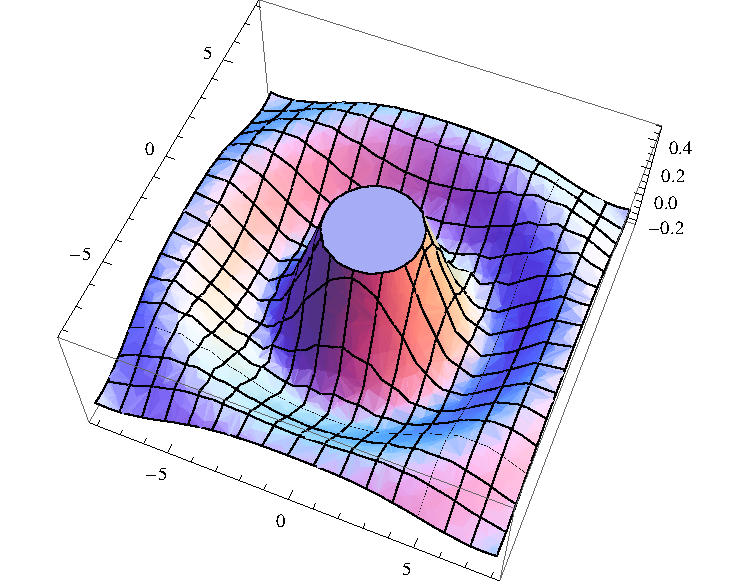
\includegraphics[width=7cm]{EjemploFigura.pdf}
%	\label{EtiquetaFigura}
%	\medskip
%	\caption*{\emph{Nota}: Esta es una nota explicativa\\ sobre la imagen (opcional)}
%\end{figure}

%\noindent En la Tabla \ref{EtiquetaDeLaTabla} ...
%\begin{table}[h!]
%\caption{Título de la tabla}
%\centering
%\begin{tabular}{c|c|c}
%	& 1 & 2 \\
%	\hline
%	A &  &  \\
%	\hline
%	B &  &  \\
%\end{tabular}
%\label{EtiquetaDeLaTabla}
%\medskip
%\caption*{\emph{Nota}: Nota de la tabla (opcional)}
%\end{table}


%\section{Cómo citar}\label{EtiquetaDeSeccion23}
%\begin{itemize}
%	\item \textbf{Citas cortas} (hasta 40 palabras):Se incluyen en el texto con comillas.
%	\item \textbf{Citas largas} (más de 40 palabras): Se escriben en párrafo separado sin comillas.
%\end{itemize}
%
%\subsection{\emph{apacite}}
%\noindent Para citar en formato APA, puede usarse el paquete \emph{apacite}. Algunas opciones de citación pueden hacerse con los comandos que se presentan en la Tabla \ref{ComandosApacite}; puede consultar \cite{meijer2013apacite} para la información completa de la documentación del paquete.

%\begin{table}[h!]
%\caption{Algunos comandos del paquete \emph{apacite} }
%\centering
%\scriptsize
%	\begin{tabular}{ll}
%		\hline
%		\textbf{Texto plano}&\textbf{Produce}\\
%		\hline
%		\verb|\cite{RudinKEY} afirma que|&\cite{RudinKEY} afirma que \\
%		\verb|\cite[p.123]{RudinKEY} afirma que|&\cite[p.123]{RudinKEY} afirma que\\
%		\verb|Como se pude ver en  \citep{RudinKEY}|&Como se pude ver en  \citep{RudinKEY}\\
%		\verb|\citealp{RudinKEY}|&\citealp{RudinKEY}\\
%		\verb|Ver Rudin \citeyearpar {RudinKEY}|&Ver Rudin \citeyearpar {RudinKEY}\\
%		\verb|Como se pude ver en  \citet{RudinKEY}|&Como se pude ver en  \citet{RudinKEY}\\
%		\verb|Como se pude ver en  \citetext{RudinKEY}|&Como se pude ver en  \citetext{RudinKEY}\\
%		\verb|Puede consultar \citeauthor {RudinKEY}|&Puede consultar \citeauthor {RudinKEY}\\
%		\verb|Confrontar Lamport \citeyear {RudinKEY}|&Confrontar Lamport \citeyear {RudinKEY}\\
%		\hline
%	\end{tabular}
%\label{ComandosApacite}
%\medskip
%\caption*{\emph{Nota}: Tabla extraída de \citet[p. 50]{WunschKEY}.}
%\end{table}

%\subsection{Citas textuales}

%\begin{itemize}
%  \item \textbf{Narrativa}.

%  \underline{Cita corta}.

%   Como menciona \cite{apostol1976analisis}, ``\emph{la idea de expresar geométricamente los números complejos como puntos de un plano fue formulada por Gauss en su disertación de 1799 e, independiente, por Argand en 1806.}'' (p. 21). Sin embargo ...

%  \underline{Cita larga}

%  Como menciona \cite{apostol1976analisis}:
%  \begin{itemize}
%    \item [] La idea de expresar geométricamente los números complejos como puntos de un plano fue formulada por Gauss en su disertación de 1799 e, independiente, por Argand en 1806. Más tarde Gauss ideó la expresión un tanto desafortunada de ''número complejo''. Los números complejos admiten otras representaciones geométricas. En vez de utilizar puntos de un plano, se pueden utilizar puntos de otras superficies. (p. 22)
%  \end{itemize}



%  \item \textbf{Con paréntesis}.

%  Los números complejos, pueden representarse como puntos de un plano, ``\emph{la idea de expresar geométricamente los números complejos como puntos de un plano fue formulada por Gauss en su disertación de 1799 e, independiente, por Argand en 1806.}'' \cite[p. 21]{apostol1976analisis},

%\end{itemize}

%\subsection{Citas parafraseadas}
%\begin{itemize}
%  \item \textbf{Narrativa}.

%  De acuerdo a \cite{apostol1976analisis}, otra representación geométrica de los números complejos es la llamada \textbf{proyección estereográfica} que consiste en proyectar los puntos del polo norte de la esfera sobre el plano tangente en el polo de dicha esfera. (p. 22)
%  \item \textbf{Con paréntesis}.

%  Otra representación geométrica de los números complejos es la llamada \textbf{proyección estereográfica} que consiste en proyectar los puntos del polo norte de la esfera sobre el plano tangente en el polo de dicha esfera.\cite[p. 22]{apostol1976analisis}
%\end{itemize}



